\section{From \acs{CAD} to Voxels}
\todo[inline]{Include a super-diagram of the classes being used}
\label{sec: CADToVoxels}
One of the hurdles with most state-of-the-art open source topology optimization tools is their input format, where many of them (including ToPy, our topology optimizer of choice) require input to be specified as a 3-dimensional voxel grid. Presence (or absence) of material in these voxels is defined by a boolean variable, and boundary conditions are imposed on the appropriate locations. An example of voxelized data can be seen in \autoref{fig: voxelOpenCascade}. %Since there is a variety of toolboxes available which are able to perform a voxelization of common CAD input files, we did not implement one of our own but rather adapted one of the open source tools. %This section describes how we overcame this hurdle of converting CAD representations to voxelized input.

\subsection{Specification of Boundary Conditions for the Input Geometry}
\label{sec: GeomCreation}

\begin{figure}
\centering
  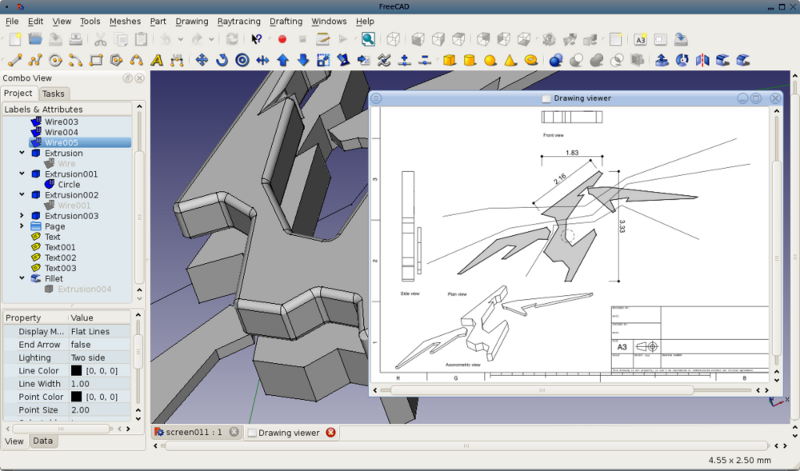
\includegraphics[scale=0.75]{Pictures/CADToVoxel/FreeCAD.png}
\caption{The FreeCAD workbench. FreeCAD is an open-source CAD modeling software, and is the primary CAD tool used in this project. Figure from \cite{FreeCAD}}
\label{fig: freeCAD}
\end{figure}

As pointed out in the \ref{sec:CADbackg}, STEP and IGES files can store color information for each face. This is the attribute that is used to specify the identity of the face, and can be modified using standard CAD design software such as FreeCAD (see \cite{FreeCAD}). When analysing a structural problem, a designer typically needs to provide information on up to five parameters:

\begin{itemize}
	\item \textbf{Optimized domain}: This refers to the main geometry that needs to be optimised. These faces are simply colored absolute white, i.e. $(255, 255, 255)$.
	\item \textbf{Fixture faces}: These faces of the geometry are meant to be fixed in space, and undergo zero displacement. These faces are colored absolute red, i.e. if the color space of red ranges in {$[0, 255]$}, then the face is assigned the extremum $255$. The blue and green color components are set to $0$. Thus, the color array is set to $(255, 0, 0)$. These are also stored in the file holding the optimized domain.
	\item \textbf{Load faces and load value}: These faces bear the forces acting on the body. Loads are three-dimensional, and can take both positive and negative values depending on their direction. To accommodate all possibilities, each color component (i.e. red, blue and green) is assigned a direction ($x$, $y$, and $z$). The range $(0, 255)$ is split in two: $(0, 127]$ representing the negative force range and $[128, 255)$ representing the positive force range. The color is then offset by $-127$. 

Of course, force values may also lie outside the offset color range, i.e $(-\infty, -127] \cup [128, \infty)$. The user then needs to scale the required force to fit in the color range, and provide a scaling factor as an input.

For example, to assign a force value of $(-200.5, 172.0, -10.75)$:

\begin{table}[h!]
	\begin{center}
		\caption{Fitting a force value to a color}
		\label{LoadFaceExample}
		\begin{tabular}{cccc}
			\toprule
			{\small Original vector} & {\small Scaling factor} & {\small Modified vector} & {\small Final color}\\
			\midrule
			$-200.5$ & $0.628428928$ & $-126$ & $1$\\
			$172.0$  & $0.628428928$ & $108$  & $235$\\
			$-10.75$ & $0.628428928$ & $-7$   & $120$\\
			\bottomrule
		\end{tabular}
	\end{center}
\end{table}

The load faces are given in a specified input file such that for example inner loads can be described.

	\item \textbf{Non-changing geometry}: Sometimes, certain parts of the geometry cannot accommodate changes. This could be for several reasons, for example, due to compatibility issues with other components. To define the geometry accurately and independently of the main geometry, it is provided in a distinguished file.% These faces are marked with absolute green, i.e. $(0, 255, 0)$.
	\item \textbf{Solution limits:} Describes a bounding box geometry referring to the area from which we take the optimized solution. Since this domain may be different from the main geometry it is also given in an additional file.
\end{itemize}

\autoref{fig: CADTopInputFiles} illustrates in more detail how the inputs needs to be defined to describe the constraint geometry. 

%The user must save the CAD file in both STEP and IGES formats. This is necessary due to some issues with the face extraction process in OpenCascade - the IGES format allows for proper face extraction, but color detection works only for the STEP format. Also, the files should be saved in the same directory, and have the same name.
\begin{figure}[ht]
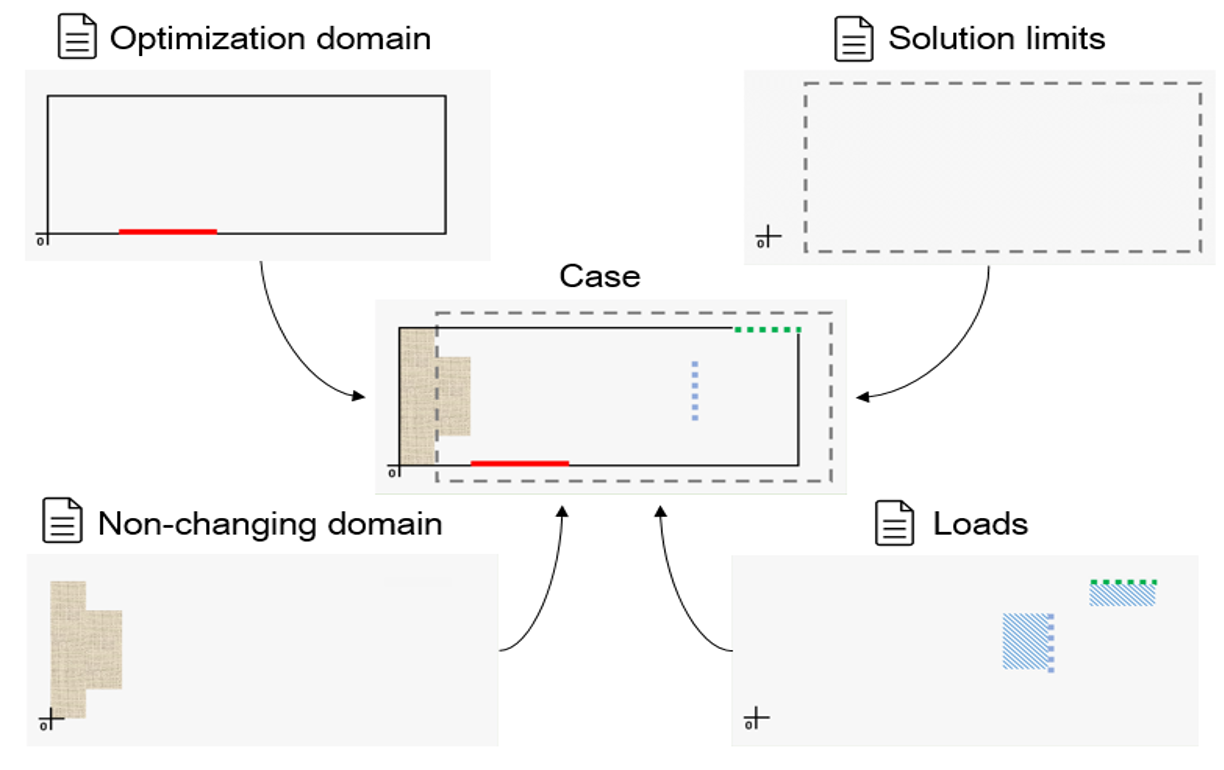
\includegraphics[width=\textwidth]{Pictures/four_files.png}
\caption{Assume the input file is called "input{\_}file". The optimization domain(top left) describes the main geometry and has to be provided in files "input{\_}file".step and "input{\_}file".iges-- .step storing the structural description while .iges holds the color information. Also the fixture faces are stored in these files. The solution limits are given in a file "input{\_}file"{\_}toOptimize.step (top right). Similarly, the non-changing domain stored as "input{\_}file"{\_}Fixed.step (bottom left). Finally, also the loads are specified in a seperate input file named "input{\_}file"{\_}load.step (bottom right).}
\label{fig: CADTopInputFiles}
\end{figure}


\input{CADImpl/FaceExtration}

\subsection{Voxelization}
\label{sec: Voxelization}

\tododone[inline]{Severin: Describe the voxelization process. Explain concept of refinement.}
%what is voxelisation
As pointed out in section \ref{sec:TopOpt} a very common formulation of topology optimization deals with regions that are specified as filled or empty. The minimum compliance problem is then solved on a discretized grid; the most common one is a volume raster in the form of cubes - so called voxels. Since ToPy requires a voxel grid in their input format, the next step is to render the geometry with a 3D raster of voxels.  

As described in the previous section, the geometry shape and faces for each boundary condition type, are stored in OpenCascade through the internal data type \lstinline|TopoDSShape|. As one can see in the UML Diagram \ref{fig: umlCADToVoxel} the \lstinline|voxelise| function is called internally by \lstinline|CADTOVoxel| -- for the shape and each faces separately. The voxelisation is then performed as follows: 
\begin{enumerate}
\item In order to combine the 3D voxel raster consistently, a bounding box is introduced. As a consequence the same coordinate system is used and voxel numbers are consistent between different voxelization types (faces and shapes). 
\item In each dimension $2^n*l_d$ voxels are created, where $n$ is the user specified refinement level and $l_d$ is the size of the bounding box in the respective dimension $d$
\item Voxelization is performed with the OpenCascade  \lstinline|Voxel_FastConverter.hxx| class creating a \lstinline|VoxelShape|
\end{enumerate}
\tododone[inline]{OpenCascade TopoBoolDS shape}

Consequentially, a 3D boolean voxel raster is created for each type -- since boundary conditions may consist of more than one face, they are voxelized separately and lists of \lstinline|VoxelShape| are created. 

\subsection{Construction of ToPy Input File}
\label{sec: ToPyInputConstruction}

\todo[inline]{Explain the difference in the coordinate system of ToPy. Explain the mirroring of directions being done in the ToPyWriter.}


\begin{figure}
\centering
  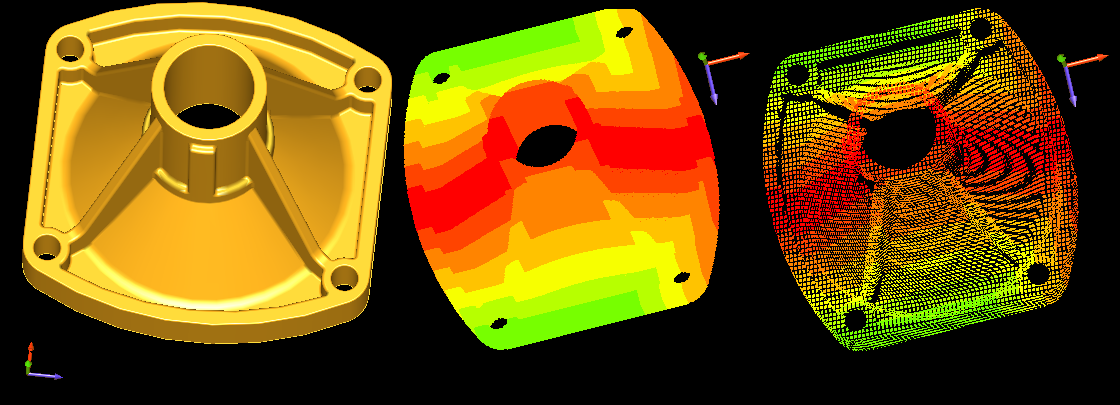
\includegraphics[scale=0.3]{Pictures/CADToVoxel/voxels_wp_image005.png}
\caption{A shape and its voxel representation. \emph{Leftmost picture}: The original parametrized shape. \emph{Rightmost picture}: The voxel representation. Picture from OpenCascade \cite{OpenCascade}.}
\label{fig: voxelOpenCascade}
\end{figure}

\begin{figure}
\centering
\begin{subfigure}{
  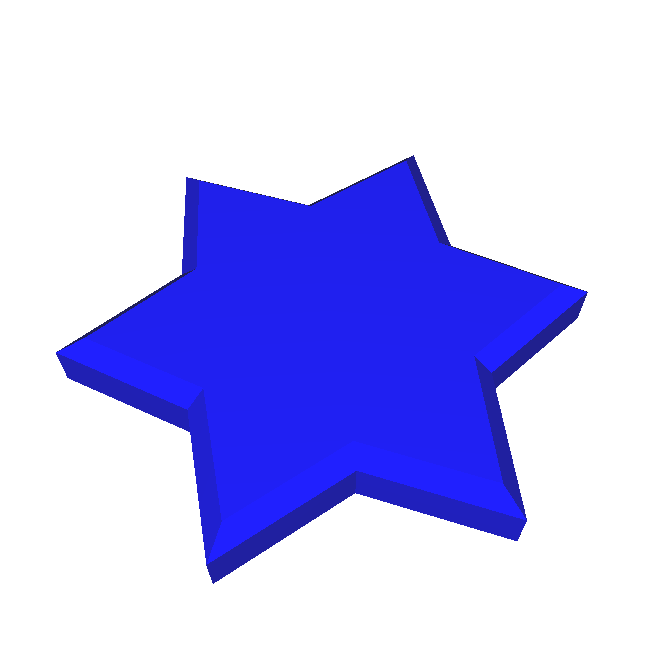
\includegraphics[width=.2\linewidth]{Pictures/STLToVoxels/Star_STL.png}}
\end{subfigure}
\begin{subfigure}{
  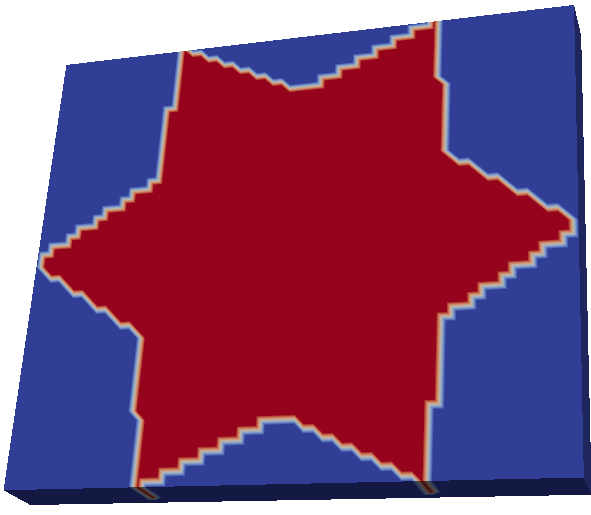
\includegraphics[width=.2\linewidth]{Pictures/STLToVoxels/Star_VTK_Trans.png}}
\end{subfigure}
\caption{The STL geometry of a star (left) and its voxelized form (right) obtained via the CVMLCPP voxelizer, visualized by Paraview \cite{Paraview}.}
\label{fig: voxelizerStar}
\end{figure}


